\chapter{Literature review}

\section{TeraRanger}
TeraBee offers an off-the-shelf solid-state LIDAR system with the purpose of collision avoidance for drones.
In their solution 8 sensors are positioned around a vertical axis with a controller board in the middle. 
TeraRanger's interface is compatible with PixHawk 4 flight controller board and PX4 flight controller 
software that makes integration easy.

Each block of the array is a standalone LIDAR sensor, that can be used separately and supports different
mount configurations. The company offers a long-range and fast-ranging version of these sensors, depending 
on the type an update rate of 320 Hz can be achieved. The fact that system comes with a ROS package and a 
2$^{\circ}$ field of view makes it a good candidate for indoor mapping in two dimensions. The price of this setup 
starts from 599 euro. \cite{TerabeeTeraRanger}

\begin{figure}[!ht]
    \centering
    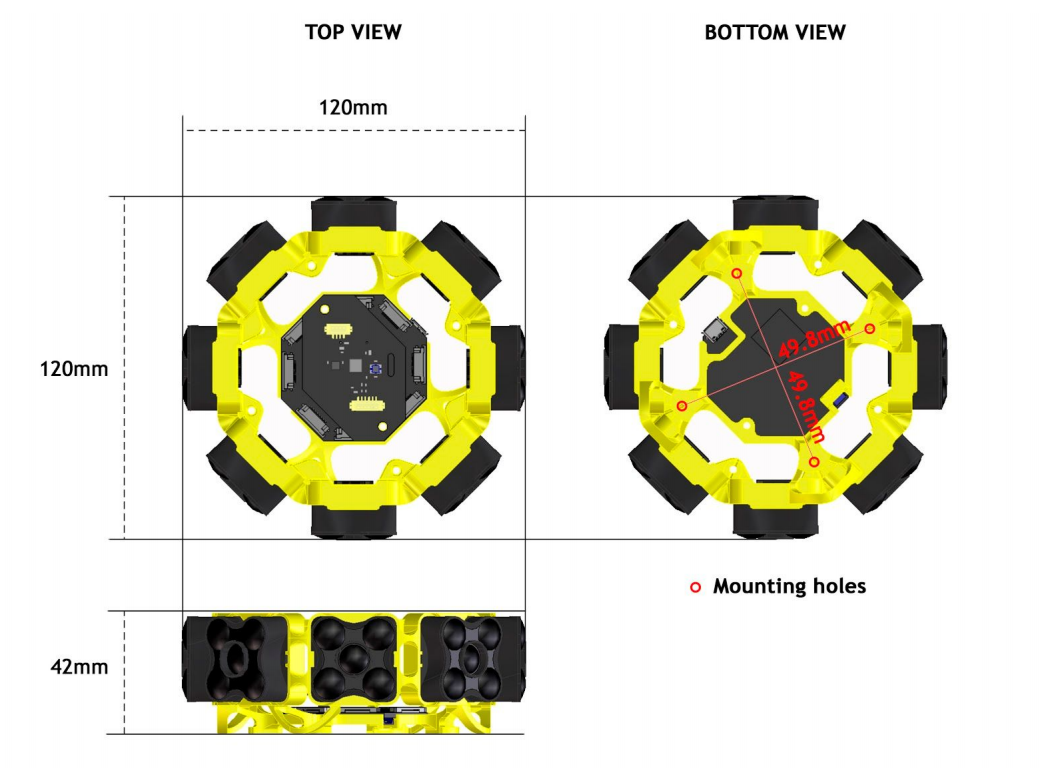
\includegraphics[width=50mm, keepaspectratio]{figures/tera_ranger_tower.png}\hspace{1cm}
    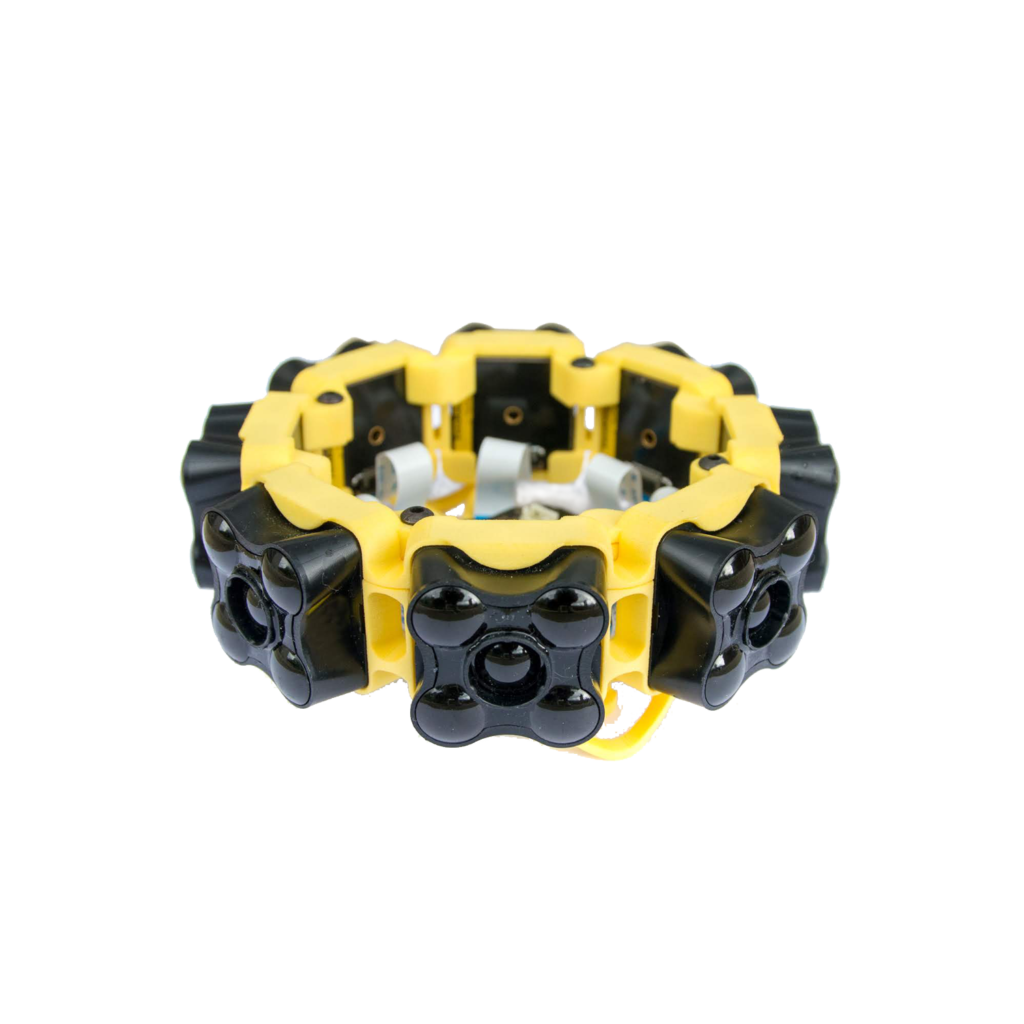
\includegraphics[width=50mm, keepaspectratio]{figures/tera_ranger_tower_2.png}
    \caption{Terabee TeraRanger Tower Evo dimensions}
    \label{fig:teraranger_dimensions}
\end{figure}

\begin{table}[ht]
	\footnotesize
	\centering
	\begin{tabular}{ l c c }
		\toprule
		                & Long-range                                & Fast-ranging \\
		\midrule
		Range           & 0.5m up to 60m                            & 0.75m up to 8m \\
		Update rate     & 120Hz/sensor                              & 320Hz/sensor\\
		Field of View   & 2$^{\circ}$                                        & 2$^{\circ}$\\
		Accuracy        & $\pm 4cm$ in the first 14m, 1.5\% above   & $\pm 12cm$\\
		\bottomrule
	\end{tabular}
	\caption{TeraRanger Tower Evo specifications}
	\label{tab:tera_ranger_features}
\end{table}


\section{Crazyflie 2.0 Multi-ranger deck}
\section{3D LIDAR SLAM Intergation with GPS/INS for UAVs in Urban GPS-Degraded Environments}